\chapter{Metodologia de pesquisa}

Segundo \citeonline[pág.~2]{rodrigues2007},a pesquisa deve conter um conjunto de abordagens, técnicas e processos para formular e resolver problemas do mundo real de maneira organizada e sistemática.

Para que uma metodologia de pesquisa fique bem estruturada é necessário responder como os objetivos serão alcançados e  como será realizada a resolução do problema de pesquisa. Para isso, deve-se classificar a pesquisa, identificar as atividades e estabelecer como as atividades serão executadas \cite{forcon2014}.

\section{Classificação da Pesquisa}

Segundo \citeonline[pág.~41]{gil2008}, a metodologia de pesquisa é classificada através de critérios bem definidos com base em seus objetivos e procedimentos técnicos.

 É usual a classificar uma pesquisa com base em seus objetivos em três grandes grupos: exploratórias, descritivas e explicativas \cite[pág.~41]{gil2008}

\begin{citacao}
“Pesquisas exploratórias têm como preocupação central identificar os fatores que determinam ou que contribuem para a ocorrência dos fenômenos. Esse é o tipo de pesquisa que mais aprofunda o conhecimento da realidade, porque explica a razão, o porquê das coisas. Por isso mesmo, é o tipo mais complexo e delicado, já que o risco de cometer erros aumenta consideravelmente” \cite[pág.~43]{gil2008}.
\end{citacao}

A pesquisa é classificada com base em procedimentos técnicos em quantitativa e qualitativa. A pesquisa quantitativa traduz em números os estudos realizados e se utiliza técnicas estatísticas para comprovar os fatos \cite[pág.~9]{rodrigues2007}

Segundo \cite[pág.~2]{bandeira2012}, a pesquisa experimental é um tipo de pesquisa quantitativa e visa identificar relações causais entre duas ou mais variáveis, através do método experimental. Esse método implica em três procedimentos básicos: variar a causa, controlar variáveis interferentes e medir a causa.

Considerando os objetivos de estudo desse TCC, será incorporada a pesquisa exploratória com o intuito de evidenciar os possíveis fenômenos que se repetem no Mercado de Moedas. Em relação aos procedimentos técnicos, será realizada a pesquisa quantitativa experimental para evidenciar como será solucionado o problema de pesquisa.

\section{Atividades da Pesquisa}

É necessário evidenciar na metodologia de pesquisa quando começam as atividades e quais são as coordenadas para que as mesmas sejam cumpridas \cite{forcon2014}.

A figura \ref{metodologia} evidencia como estão organizadas as atividades deste TCC.

\begin{figure}[H]
\centering
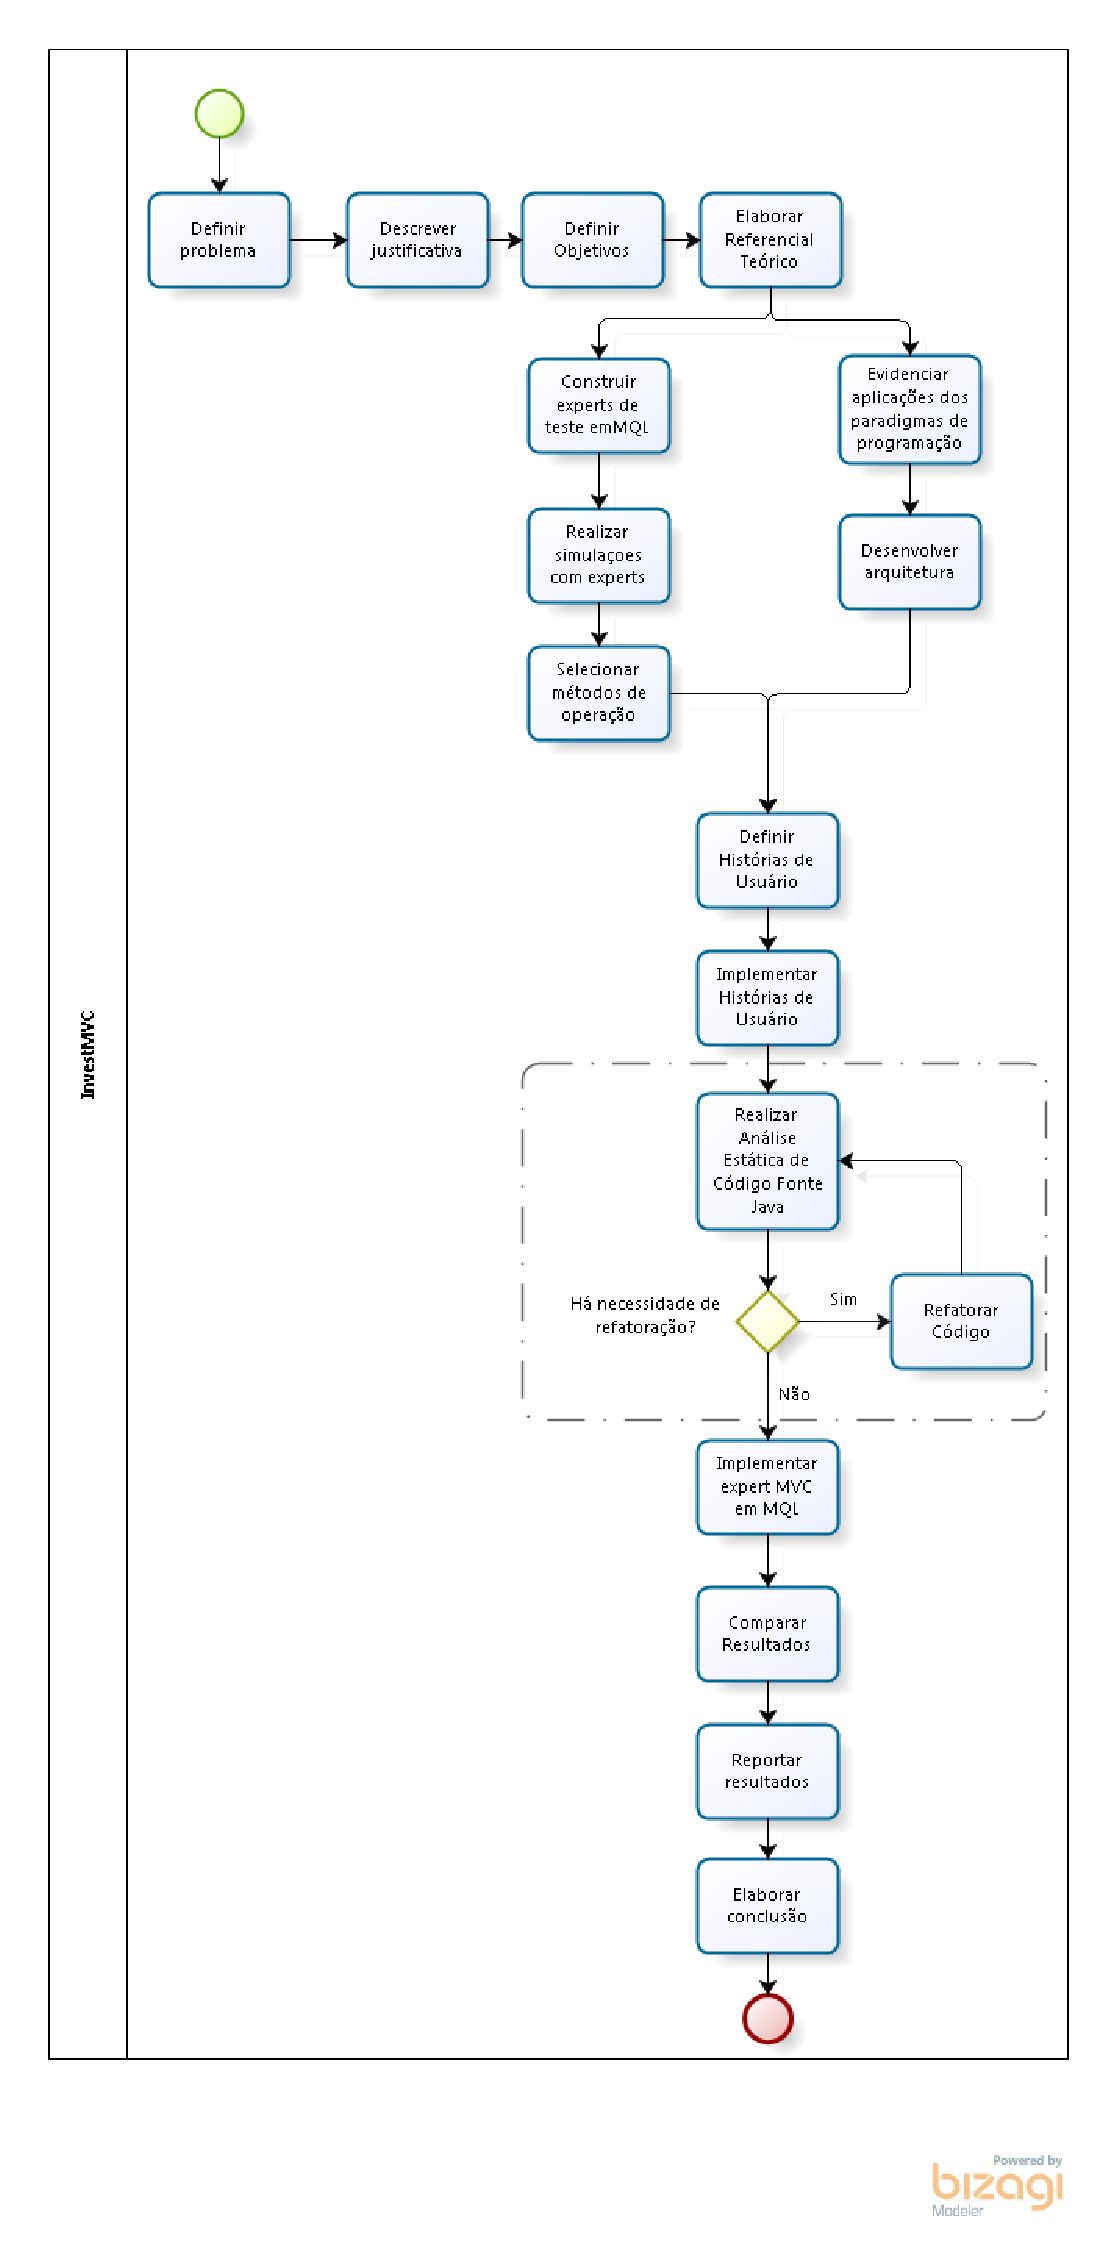
\includegraphics[width=0.7\textwidth]{figuras/metodologia}
\caption{Atividades da Pesquisa.} 
\label{metodologia}
\end{figure}

\subsection{Descrição dos Objetivos das Atividades de Pesquisa}

A tabela \ref{atividadeMetologia}  evidencia cada atividade da pesquisa e o objetivo de cada atividade.

\begin{table}[H]
\caption{Atividades e objetivos da pesquisa}
\begin{center}
    \begin{tabular}{ | c | c |}
    \hline
    \textbf{Atividade} & \textbf{Objetivo} \\ \hline
	Definir problema & Definir o problema de pesquisa do TCC.\\ \hline
	Descrever justificativa & Com base no problema de pesquisa, deve-se justificar a relevância do trabalho proposto.\\ \hline
	Elaborar referencial teórico & Com base na literatura, descrever os conceitos chaves como Contexto Financeiro, Paradigmas de Programação e Qualidade de Software.\\ \hline
	Construir experts em mql & Implementar expert Fibonacci.mql, MinimosQuadrados.mql, CorrelacaoLinear.mql, Estocastico.mql, MediaMovel.mql. \\ \hline
	Realizar experimento com experts & Definir critérios de entrada e saída para cada expert e realizar a simulação de cada expert no Mercado de Moedas durante o perído de 2 anos (agosto 2012-2014).\\ \hline
	Selecionar métodos de operação & Selecionar os métodos (Fibonacci, Mínimos Quadrados, Correlação Linear, Estocástico ou Média Móvel) que obtiverem lucro durante o período de simulação.\\ \hline
	Evidenciar aplicações paradigmas de programação & Evidenciar aplicações dos paradigmas: funcional, lógico, estruturado e multiagente.\\ \hline
	Desenvolver arquitetura & Desenvolver a arquitetura da ferramenta MVC no intuito de evidenciar decisões sobre a organização do sistema.\\ \hline
	Definir Histórias de Usuário & Definir o conjunto de funcionalidades e pontuar cada História, seguindo a sequência de Fibonacci para realizar a pontuação.\\ \hline
	Implementar Histórias de Usuário & Desenvolver as Histórias de Usuário que foram definidas.\\ \hline
	Realizar Análise Estática de Código Fonte & Realizar a análise estática de código fonte para aferir o nível de qualidade do código fonte da ferramenta MVC.\\ \hline
	Implementar expert em mql & Implementar toda a lógica da ferramenta MVC em linguagem mql.\\ \hline
	Comparar resultados monetários expert mql e ferramenta mvc & Comparar os resultados monetários do expert em mql com a ferramenta MVC durante um tempo a se determinado de operação.\\ \hline
	Reportar resultados & Registrar os resultados da comparação do desempenho da ferramenta MVC e do expert em mql.\\ \hline
	Elaborar conclusões & Desenvolver as conclusões do TCC.\\ \hline
    \end{tabular}
    \end{center}
\label{atividadeMetologia}
\end{table}

\section{Execução da Pesquisa}

Scrum é uma metodologia de desenvolvimento fundada na teoria do controle de processos empíricos. O empirismo afirma que conhecimento vem da experiência. As decisões são tomadas com base na experiência em que se tem de um determinado assunto. Scrum emprega uma abordagem iterativa e incremental para otimizar a previsibilidade e controle de riscos da execução de um projeto. Existem três pilares sustentam qualquer implementação de controle de processos empíricos: transparência, inspeção e adaptação \cite[pág.~4]{schwaber2013}.

Nesse TCC, vertentes defendidas pelo Scrum serão adaptadas e incorporadas a metodologia de pesquisa. Os produtos de  trabalho serão alocados e desenvolvidos em Sprints (intervalo de tempo de 1 a 4 semanas). Durante a execução de uma Sprint, serão usadas adaptações que forem necessárias para que os artefatos e  produtos de software tenham a maior qualidade possível.

\chapter{Cronograma InvestMVC}

A tabela \ref{cronograma} mostra quais são as atividades em cada Sprint e a duração da mesma. O cronograma detalhado encontra-se no apêndice A - Cronograma InvestMVC.

\begin{table}
\caption{Cronograma simplificado}
\begin{center}
    \begin{tabular}{  | p{2cm} | p{8cm} | p{2cm}| p{2cm} |}
    \hline
    \textbf{Sprint} & \textbf{Atividades} & \textbf{Data de início} & \textbf{Data de finalização}\\ \hline
    Sprint 1 & \begin{enumerate}
    \item Construir introdução
    \item Implementar Métodos Numéricos
    \end{enumerate} & 10/08/2014 & 31/08/2014\\ \hline
    
    Sprint 2 & \begin{enumerate}
    \item Construir Referencial Teórico Paradigmas de Programação
    \item Adaptar Métodos Numéricos
    \item Prototipar View Projeto
    \item Construir Referencial Teórico Métodos Numéricos
    \end{enumerate} & 01/09/2014 & 15/09/2014\\ \hline
    
    Sprint 3 & \begin{enumerate}
    \item Refinar Referencial Teórico Paradigmas
    \item Construir Referencial Teórico de Contexto Financeiro
    \item Revisar Referencial Teórico Métodos Numéricos
    \end{enumerate} & 16/09/2014 & 30/09/2014\\ \hline
    
    Sprint 4 & \begin{enumerate}
    \item Realizar Experimentos Métodos de Operação
    \item Revisar Referencial Teórico Contexto Financeiro
    \item Desenvolver Experts em MQL4
    \end{enumerate} & 01/10/2014 & 15/10/2014\\ \hline
    
    Sprint 5 & \begin{enumerate}
    \item Descrever Metodologia de Pesquisa
    \item Realizar Experimentos Métodos de Operação
    \item Evidenciar Aplicações Paradigmas de Programação
    \end{enumerate} & 16/10/2014 & 31/10/2014\\ \hline
    
    Sprint 6 & \begin{enumerate}
    \item Definir Backlog de Histórias de Usuário
    \item Verificar Qualidade de código fonte
    \end{enumerate} & 01/11/2014 & 10/11/2014\\ \hline
    \end{tabular}    
\end{center}
\label{cronograma}
\end{table}
